\vspace{-0.6em}
\section{Benchmark Design and Dataset Construction}
\label{sec:dataset}
\vspace{-0.6em}
\subsection{Benchmark Design Principles: What Tasks are We Looking for?}
\label{sec:design-principles}

The benchmark is defined by three high-level requirements. They determine which workflows are
admitted into the dataset and which are rejected in the public submission portal:

\noindent \textbullet\ \textbf{Representativeness.} The workflow should match real professional practice and use the software that domain experts would actually use. 
\noindent For example, architectural experts would typically use \colorbox{green!8}{SolidWorks or Rhino} rather than \colorbox{red!8}{AutoCAD} to convert a 2D blueprint into a 3D model.

\noindent \textbullet\ \textbf{Complexity.} A task should be an end-to-end deliverable that would take an expert substantial time, rather than only a few UI operations. The key distinction is between a workflow and an action.

\noindent \colorbox{red!8}{\parbox{\dimexpr\linewidth-2\fboxsep\relax}{\textit{Undesired example.} ``Apply a color filter in DaVinci'' is too narrow because it's a single local edit.}}

\noindent \colorbox{green!8}{\parbox{\dimexpr\linewidth-2\fboxsep\relax}{\textit{Better example.} ``Move a running cheetah into another race video'' is suitable because it requires tracking, rotoscoping, compositing, and color matching within one coupled workflow.}}

\noindent \textbullet\ \textbf{Verifiability.} The output should admit deterministic checking or an unambiguous rubric tied to observable artifacts. The strongest case is a deterministic deliverable that can be compared directly against a reference output. When exact matching is impossible, the judgment should still reduce to a measurable artifact.

\noindent \colorbox{red!8}{\parbox{\dimexpr\linewidth-2\fboxsep\relax}{\textit{Undesired example.} ``Design an RPG game with monsters'' provides no objectively checkable target.}}

\noindent \colorbox{green!8}{\parbox{\dimexpr\linewidth-2\fboxsep\relax}{\textit{Better example.} ``Reproduce the game \textit{mota.exe} using RPGMaker XP'' is verifiable because the resulting map geometry, character attributes, and event states can be automatically compared against a reference version under identical trajectories of user operations.}}

\vspace{-0.4em}
\subsection{Benchmark Scope and Taxonomy: Which Domains Do We Cover?}
\label{sec:taxonomy}
\vspace{-0.4em}
Rather than selecting industries ad hoc or by economic ranking, we ground the ALE taxonomy in SOC 2018~\citep{bls2018soc} and O*NET~\citep{peterson2001onet}: we cluster occupations with similar software-mediated workflows into ALE industries, exclude sectors whose core work is not meaningfully digital, and group the result into \clustercount{} domains spanning \taskcount{} subdomains (Figure~\ref{fig:teaser}; full derivation in Appendix~\ref{app:taxonomy}). To enable fair cross-benchmark comparison, we map each prior benchmark's published categories (subjects, applications, repositories, or occupations) onto the same \taskcount{}-subdomain taxonomy via an LLM-assisted classifier. The result exposes a coverage gap that no existing benchmark closes: even the union of 16 major prior benchmarks leaves \textbf{13 of \taskcount{} subdomains} entirely uncovered (Table~\ref{tab:related-comparison}).

\vspace{-0.4em}
\subsection{Task Construction Pipeline: How are the Tasks Created?}
\label{sec:construction-pipeline}

\begin{figure}[htbp]
  \centering
  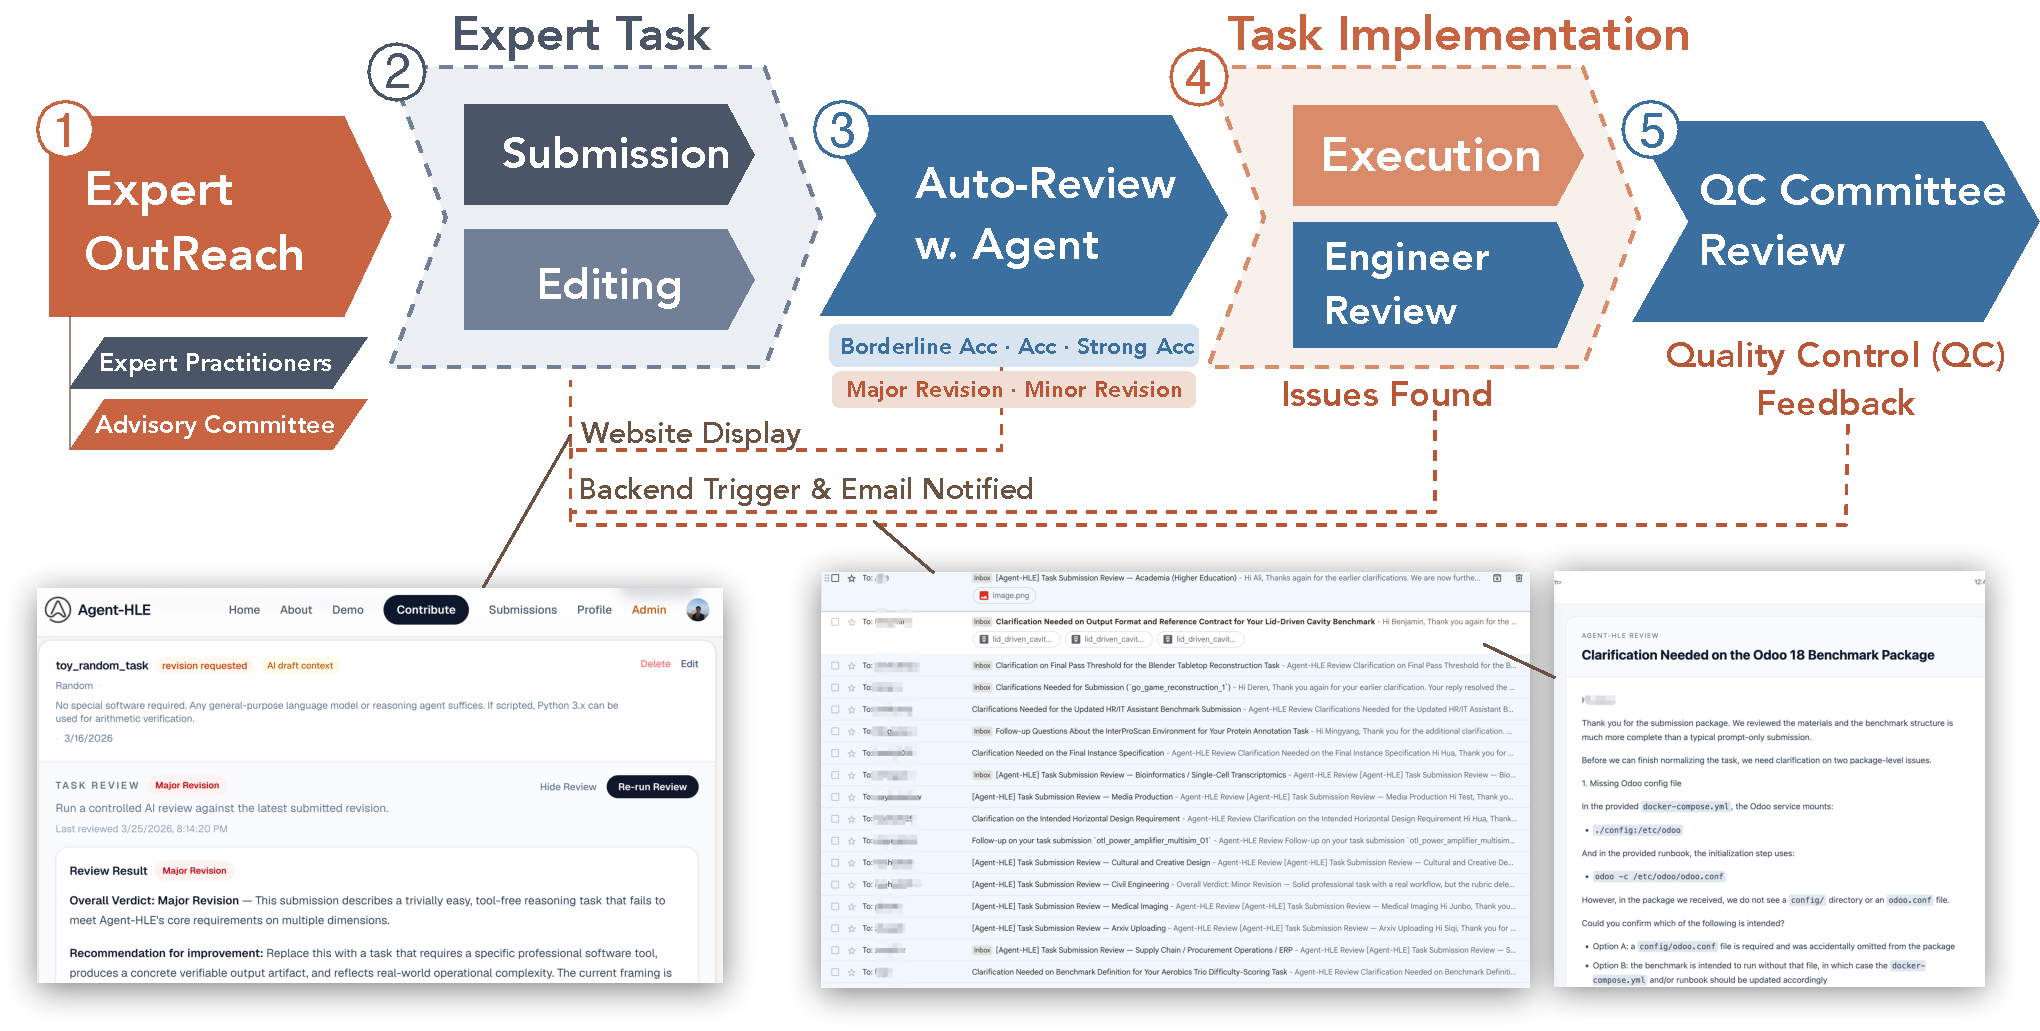
\includegraphics[width=1.0\linewidth]{figures/pipeline-flowchart}
  \caption{\textbf{Task construction pipeline.} Tasks proceed from expert sourcing through submission, first-pass review, engineering implementation, and final quality control.}
  \label{fig:pipeline}
  \vspace{-0.3cm}
\end{figure}

\begin{wrapfigure}{r}{0.5\textwidth}
  \vspace{-0.4em}
  \centering
  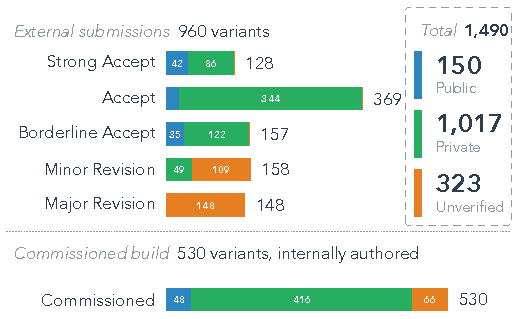
\includegraphics[width=\linewidth]{figures/build_distribution/panel_a/panel_a_compact.pdf}
  \caption{\textbf{Provenance and review yield.} The \totalvariants{} task instances split into 960 external submissions (top, by first-pass review verdict) and 530 commissioned tasks (bottom). Each bar is segmented by release state: \publictaskcount{} public, 1{,}017 private, and 323 unverified pending QC.}
  \label{fig:pipeline-yield}
  \vspace{-0.5em}
\end{wrapfigure}
Tasks in ALE cannot be crowdsourced from lay workers; they must arise from the actual routines of domain professionals and undergo rigorous screening to guarantee authenticity, complexity, and technical executability. We therefore employ a staged construction protocol (Figure~\ref{fig:pipeline}) with five gates. \textit{Expert sourcing} recruits domain specialists through an advisory committee of industry practitioners, ensuring coverage across the taxonomy. \textit{Task submission} routes proposals through a dedicated web portal (\url{https://agents-last-exam.org/submit/new/form}), where experts upload past projects that took them days or weeks of professional work and AI-assisted tools help refine each proposal until five core components are fully specified: a natural-language description, input files, target software, expected deliverable, and evaluation specification.
\textit{First-pass review} screens submissions with conference-style decisions (\texttt{major / minor revision}, \texttt{borderline accept}, \texttt{accept}, \texttt{strong accept}); revisions loop back to the expert. \textit{Task implementation} converts accepted specifications into runnable assets, provisioned software containers, and codified evaluation logic, with engineer dry-runs and automatic routing back to the expert when gaps are found. \textit{Final QC} is a peer review by the expert committee that verifies reference-output correctness, calibration of evaluation bounds (neither impossibly narrow nor spuriously permissive), and sufficiency of context before the task is admitted. More details are deferred to Appendix~\ref{app:construction-pipeline}.

\noindent \textbf{Public/private release strategy.}
Benchmark contamination, whether through pre-training data overlap or task-specific optimization, is a central threat to the long-term validity of any public evaluation.
ALE addresses this by releasing only \publictaskcount{} of the \totalvariants{} task instances ($\sim$10\%) publicly, with the remainder held in a private pool (Figure~\ref{fig:pipeline-yield}).
ALE is further designed for \emph{rolling evaluation}: private task instances will periodically rotate into the public set while retired public tasks are replaced, maintaining an uncontaminated evaluation surface over successive model generations.
Appendix~\ref{app:fullpool} verifies empirically that the public subset is representative of the full pool.
